%-----------------------------------------------------------------------------
%
%               Template for sigplanconf LaTeX Class
%
% Name:         sigplanconf-template.tex
%
% Purpose:      A template for sigplanconf.cls, which is a LaTeX 2e class
%               file for SIGPLAN conference proceedings.
%
% Guide:        Refer to "Author's Guide to the ACM SIGPLAN Class,"
%               sigplanconf-guide.pdf
%
% Author:       Paul C. Anagnostopoulos
%               Windfall Software
%               978 371-2316
%               paul@windfall.com
%
% Created:      15 February 2005
%
%-----------------------------------------------------------------------------


\documentclass[preprint]{sigplanconf}

% Tobias' default latex headers
%%%%%%%%%%%%%%%%%%%%%%%%%%%%%%%

% Add support for \includegraphics
\usepackage{graphicx}
\graphicspath{{images/}}

% Add support for todo notes
% The following code contains a variation of the great code by Antal S-Z
% in his answer to http://tex.stackexchange.com/a/6029/3954
%in TeX.SX
\usepackage{tikz}
\usetikzlibrary{calc}
\usetikzlibrary{decorations.pathmorphing}
\usepackage{soul}
\usepackage{xcolor}
\newcommand*\numcircled[1]{\raisebox{1pt}{\tikz[baseline=(char.base)]{
                \node[shape=circle,draw,inner sep=1.0pt] (char) {\footnotesize #1};}}}

\newlength\LineWidth
\newlength\Amplitude
\newlength\SegLength

\setlength\LineWidth{0.4pt}
\setlength\Amplitude{1pt}
\setlength\SegLength{5pt}

\definecolor{HLcolor}{RGB}{240,0,0}

\makeatletter
\newcommand{\removelatexerror}{\let\@latex@error\@gobble}
\makeatother

\usepackage{xparse}

\newcommand\tikzmark[1]{%
  \tikz[overlay,remember picture] \node (#1) {};}

\makeatletter
\newcommand{\highlight@DoHighlight}{
  \draw[HLcolor,line width=\LineWidth,decorate,decoration={zigzag,amplitude=\Amplitude,segment length=\SegLength}]  ($(begin highlight)+(0,-2pt)$) -- ($(end highlight)+(0,-2pt)$) ;
}

\newcommand{\highlight@BeginHighlight}{
  \coordinate (begin highlight) at (0,0) ;
}

\newcommand{\highlight@EndHighlight}{
  \coordinate (end highlight) at (0,0) ;
}

\newdimen\highlight@previous
\newdimen\highlight@current

\DeclareRobustCommand*\highlight[1][]{%
  \SOUL@setup
  %
  \def\SOUL@preamble{%
    \begin{tikzpicture}[overlay, remember picture]
      \highlight@BeginHighlight
      \highlight@EndHighlight
    \end{tikzpicture}%
  }%
  %
  \def\SOUL@postamble{%
    \begin{tikzpicture}[overlay, remember picture]
      \highlight@EndHighlight
      \highlight@DoHighlight
    \end{tikzpicture}%
  }%
  %
  \def\SOUL@everyhyphen{%
    \discretionary{%
      \SOUL@setkern\SOUL@hyphkern
      \SOUL@sethyphenchar
      \tikz[overlay, remember picture] \highlight@EndHighlight ;%
    }{%
    }{%
      \SOUL@setkern\SOUL@charkern
    }%
  }%
  %
  \def\SOUL@everyexhyphen##1{%
    \SOUL@setkern\SOUL@hyphkern
    \hbox{##1}%
    \discretionary{%
      \tikz[overlay, remember picture] \highlight@EndHighlight ;%
    }{%
    }{%
      \SOUL@setkern\SOUL@charkern
    }%
  }%
  %
  \def\SOUL@everysyllable{%
    \begin{tikzpicture}[overlay, remember picture]
      \path let \p0 = (begin highlight), \p1 = (0,0) in \pgfextra
        \global\highlight@previous=\y0
        \global\highlight@current =\y1
      \endpgfextra (0,0) ;
      \ifdim\highlight@current < \highlight@previous
        \highlight@DoHighlight
        \highlight@BeginHighlight
      \fi
    \end{tikzpicture}%
    \the\SOUL@syllable
    \tikz[overlay, remember picture] \highlight@EndHighlight ;%
  }%
  \SOUL@
}
\makeatother

\DeclareDocumentCommand\MarkText{O{red}O{1pt}O{5pt}m}{%
  \colorlet{HLcolor}{#1}
  \setlength\Amplitude{#2}%
  \setlength\SegLength{#3}%
  \tikzmark{endquote}\tikzmark{beginquote}\highlight{#4}%
}
\usepackage{xargs}
\usepackage[colorinlistoftodos,prependcaption,textsize=tiny]{todonotes}
\newcommandx{\grosser}[2][1=]{#1 \todo[linecolor=red,backgroundcolor=red!25,bordercolor=red,#1]{\textbf{Tobias:} #2}}
\newcommandx{\grossermark}[2][1=]{\MarkText[red]{#2}}

%%%%%%%%%%%%%%%%%%%%%%%%%%%%%%%

% The following \documentclass options may be useful:

% preprint      Remove this option only once the paper is in final form.
% 10pt          To set in 10-point type instead of 9-point.
% 11pt          To set in 11-point type instead of 9-point.
% numbers       To obtain numeric citation style instead of author/year.

\usepackage{amsmath}

\newcommand{\cL}{{\cal L}}

\begin{document}

\special{papersize=8.5in,11in}
\setlength{\pdfpageheight}{\paperheight}
\setlength{\pdfpagewidth}{\paperwidth}

\conferenceinfo{CONF 'yy}{Month d--d, 20yy, City, ST, Country}
\copyrightyear{20yy}
\copyrightdata{978-1-nnnn-nnnn-n/yy/mm}
\copyrightdoi{nnnnnnn.nnnnnnn}

% Uncomment the publication rights you want to use.
%\publicationrights{transferred}
%\publicationrights{licensed}     % this is the default
%\publicationrights{author-pays}

\titlebanner{banner above paper title}        % These are ignored unless
\preprintfooter{short description of paper}   % 'preprint' option specified.

\title{Title Text}
\subtitle{Subtitle Text, if any}

\authorinfo{Name1}
           {Affiliation1}
           {Email1}
\authorinfo{Name2\and Name3}
           {Affiliation2/3}
           {Email2/3}

\maketitle

\begin{abstract}
This is the text of the abstract.
\end{abstract}

\category{CR-number}{subcategory}{third-level}

% general terms are not compulsory anymore,
% you may leave them out
\terms
term1, term2

\keywords
keyword1, keyword2

\section{Introduction}

The text of the paper begins here.

Some \grossermark{problematic} text which certainly also requires a comment to
be explained.\grosser{Is this correct?}.

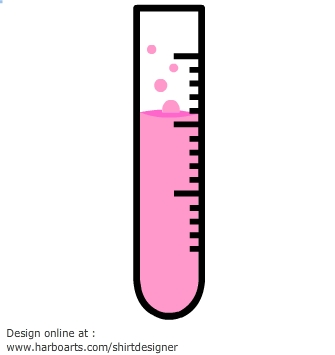
\includegraphics{example.jpg}

\appendix
\section{Appendix Title}

This is the text of the appendix, if you need one.

\acks

Acknowledgments, if needed.

% We recommend abbrvnat bibliography style.

\bibliographystyle{abbrvnat}

% The bibliography should be embedded for final submission.

\begin{thebibliography}{}
\softraggedright

\bibitem[Smith et~al.(2009)Smith, Jones]{smith02}
P. Q. Smith, and X. Y. Jones. ...reference text...

\end{thebibliography}


\end{document}
